\documentclass{article}
\usepackage{amsmath}
\usepackage{amssymb}
\usepackage{svg}
\usepackage[pdftex]{graphicx}
\usepackage[framed,numbered,autolinebreaks,useliterate]{mcode}
\lstset{breakatwhitespace=false}
\usepackage{pgfplots}

\pdfpagewidth 8.5in
\pdfpageheight 11in
\topmargin -1in
\headheight 0in
\headsep 0in
\textheight 8.5in
\textwidth 6.5in
\oddsidemargin 0in
\evensidemargin 0in 
\headheight 50pt
\headsep 0in
\footskip .75in

\title{STA 601 - Lab 7}
\author{Kedar Prabhudesai}
\date{November 1, 2013}

\begin{document}
\maketitle

\noindent {\underline{\textbf{Data Likelihood:}}}\\
\begin{eqnarray*}
L(x;\mu,\sigma) = \prod_{i=1}^{n}{\frac{1}{x_i\sigma \sqrt{2\pi}}exp\left[\frac{-(ln x_i-\mu)^2}{2\sigma^2}\right]}
\end{eqnarray*}

Let $\tau = 1/\sigma^2$\\

\begin{eqnarray*}
L(x;\mu,\tau) &=& \prod_{i=1}^{n}{\frac{\sqrt{\tau}}{x_i\sqrt{2\pi}}exp\left[\frac{-\tau(ln x_i-\mu)^2}{2}\right]}\\
\therefore L(x;\mu,\tau) &=& \frac{\tau^{n/2}}{x_i^n2\pi^{n/2}}exp\left[-\frac{\tau}{2}\sum_{i=1}^{n}{(ln x_i-\mu)^2}\right]\\
\end{eqnarray*}

\noindent {\underline{\textbf{Priors:}}}\\
\begin{eqnarray*}
\mu &\sim& \mathcal{N}(\mu_0,\tau_0)\\
\therefore p(\mu) &=& \frac{\sqrt{\tau_0}}{\sqrt{2\pi}}exp\left[\frac{-\tau_0(\mu-\mu_0)^2}{2}\right]\\
\tau &\sim& Gamma(\alpha,\beta)\\
\therefore p(\tau) &=& \frac{\beta^\alpha}{\Gamma(\alpha)}\tau^{\alpha-1}exp(-\beta\tau)
\end{eqnarray*}

\noindent {\underline{\textbf{Posterior:}}}\\
\begin{eqnarray*}
p(\mu,\tau \mid x) &\propto& L(x;\mu,\tau) \times p(\mu) \times p(\tau)\\
\therefore p(\mu,\tau \mid x) &\propto& \frac{\tau^{n/2}}{x_i^n}exp\left[-\frac{\tau}{2}\sum_{i=1}^{n}{(ln x_i-\mu)^2}\right] \times \sqrt{\tau_0}exp\left[\frac{-\tau_0(\mu-\mu_0)^2}{2}\right] \times \tau^{\alpha-1}exp(-\beta\tau)
\end{eqnarray*}

\pagebreak

\noindent {\underline{\textbf{Full Conditionals:}}}\\
\begin{eqnarray*}
p(\mu \mid \tau,x) &\propto& exp\left[-\frac{\tau}{2}\sum_{i=1}^{n}{(ln x_i-\mu)^2}\right] \times exp\left[\frac{-\tau_0(\mu-\mu_0)^2}{2}\right]\\
\therefore p(\mu \mid \tau,x) &\propto& exp\left[-\frac{\tau}{2}\sum_{i=1}^{n}{(ln x_i-\mu)^2} - \frac{\tau_0}{2}(\mu-\mu_0)^2\right]\\
\end{eqnarray*}
---------------------\\
\begin{eqnarray*}
p(\tau \mid \mu,x) &\propto& \tau^{n/2}exp\left[-\frac{\tau}{2}\sum_{i=1}^{n}{(ln x_i-\mu)^2}\right] \times \tau^{\alpha-1}exp(-\beta\tau)\\
&\propto& \tau^{\alpha + n/2 -1 }exp\left[-\frac{\tau}{2}\sum_{i=1}^{n}{(ln x_i-\mu)^2}-\beta\tau\right]\\
&\propto& \tau^{\alpha + n/2 -1 }exp\left[-\tau\left(\frac{\sum_{i=1}^{n}{(ln x_i-\mu)^2}}{2}+\beta\right)\right]\\
\therefore p(\tau \mid \mu,x) &\sim& Gamma\left(\alpha + \frac{n}{2},\frac{\sum_{i=1}^{n}{(ln x_i-\mu)^2}}{2}+\beta\right)\\
\end{eqnarray*}

In our Gibbs Sampler, we will update $\mu$ using Metropolis-Hastings and $\tau$ using the Gamma Distribution. I used the following prior parameters,\\
\begin{eqnarray*}
\mu_0 = 0,\\
\tau_0 = 0.05,\\
\alpha = 1,\\
\beta = 20.\\
\end{eqnarray*}

\noindent {\underline{\textbf{Gibbs Sampler:}}}\\

Start with \{\mu^{(0)}\}\\

\begin{itemize}
\item Sample, $\mu' \sim \mathcal{N}(\mu^{(s)},\sigma_{cand})$\\
\item Compute acceptance ratio, $r = p(\mu' \mid \tau^{(s)},x)/p(\mu \mid \tau^{(s)},x)$\\
\item Draw, $u \sim$ Uniform[$0,1$]. If $u < r,$ $\mu^{(s+1)} = \mu'$, else $\mu^{(s+1)} = \mu^{(s)}$.\\
\item Sample, $\tau^{(s+1)} \sim p(\tau \mid \mu^{(s+1)},x)$\\
\end{itemize}

\pagebreak

\noindent {\underline{\textbf{Sampling Results:}}}\\

I used a Burn-In of $2000$ trials. After much tinkering, I got good mixing for $\mu$ updates with $\sigma_{cand} = 0.5.$ We have to convert $\tau$ to $\sigma^2.$ Following are trace plots for $\mu$ and $\sigma^2.$

%\begin{center}
%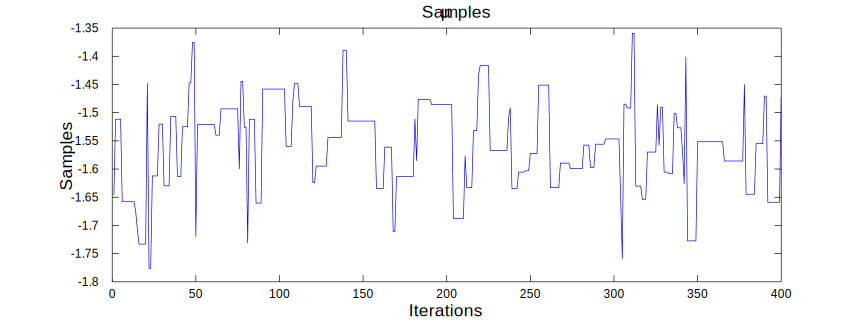
\includegraphics[scale=0.75]{muSamples.png}\\
%\end{center}
%
%\begin{center}
%\includegraphics[scale=0.75]{s2Samples.png}\\
%\end{center}




%\begin{figure}[htbp]
  %\centering
  %\includesvg{S2Samples}
  %\caption{\sigma^2 Samples}
%\end{figure}

\noindent {\underline{\textbf{Estimates and 95\% Credible Intervals for Mean and Variance:}}}\\

Mean = $e^{\mu+\sigma^2/2} \rightarrow 0.3904$ [$0.2990,0.5199$].\\

Variance = $\left(e^{\sigma^2}-1\right)e^{2\mu+\sigma^2} \rightarrow 0.4041$ [$0.1541,0.9669$].\\

\pagebreak
\noindent {\Large\underline{\textbf{Appendix:}}}\\
\lstinputlisting{C:/Users/ksp6/Documents/Classes/2013-Fall/STA601-BayesAndModStats/labs/lab7/sta601_ksp6_Lab7.m}

\end{document}